% !TeX root = ../main.tex
\section{Materials}
\label{sec:materials}

% --------------------------------------------------------
\subsection{Study area}
\label{sec:study_area}

This study covers mainland Ecuador in northwestern South America, where moist Pacific and Amazonian air masses ascending the Andes generate frequent rainfall and persistent year-round cloud cover~\citep{Bendix2006EcuadorClouds} (Fig.~\ref{fig:study_area}a). Ecuador is the world's leading supplier of balsa (\textit{Ochroma pyramidale}) timber, accounting for roughly 90\% of global supply during the 2020 wind-energy boom~\citep{CanadasLopez2019BalsaGrowth}. Commercial plantations are concentrated across the humid Pacific coastal lowlands and western Andean foothills---primarily in Los R\'ios, Santo Domingo de los Ts\'achilas, Manab\'i, Guayas, Esmeraldas, Cotopaxi, and Pichincha---at elevations of 20--700~m, mean annual temperatures of 23.5--26.7~$^{\circ}$C, and annual precipitation of 1,000--3,019~mm, with recent expansion into the Amazonian provinces of Pastaza and Napo~\citep{CanadasLopez2019BalsaGrowth}. Under these warm, humid conditions, productive stands achieve mean annual volume increments of 29--33~m$^{3}$~ha$^{-1}$~yr$^{-1}$ and reach harvestable dimensions within approximately three years~\citep{CanadasLopez2019BalsaGrowth}.

\begin{figure}[pos=!htbp]
    \centering
    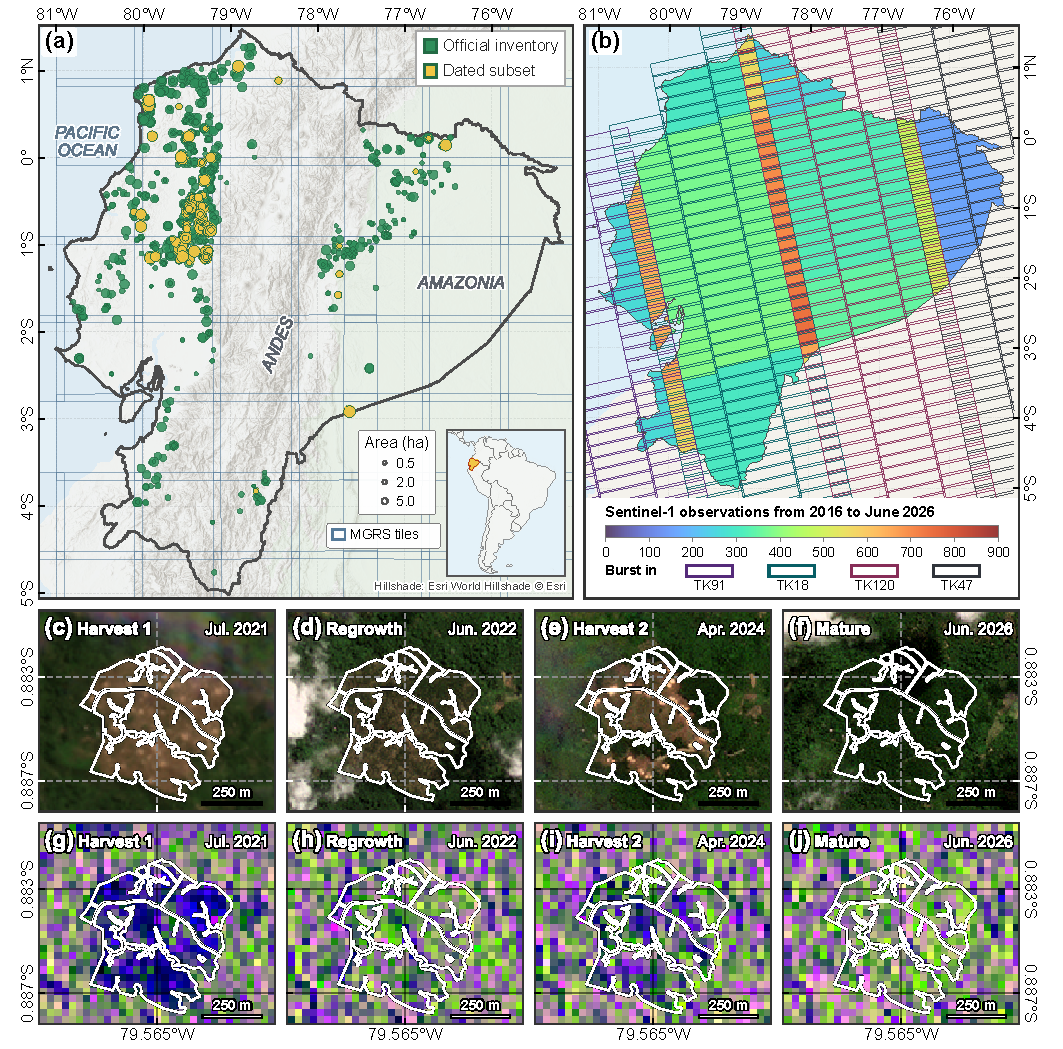
\includegraphics[width=0.96\linewidth]{figures/fig01_study_area.pdf}
    \caption{Study area and satellite observations of Ecuadorian balsa plantations. (a) Official balsa inventory and dated reference subset. (b) Cumulative ascending Sentinel-1 RTC burst observations (May 2016--June 2026) across tracks TK18, TK47, TK91, and TK120. (c--f) PlanetScope basemaps and (g--j) corresponding Sentinel-1 composites ($\mathrm{R}=\mathrm{VV}$, $\mathrm{G}=\mathrm{VH}$, $\mathrm{B}=\mathrm{VV}-\mathrm{VH}$) across two harvests and intervening regrowth.}
    \label{fig:study_area}
\end{figure}

% --------------------------------------------------------
\subsection{Satellite data}
\label{sec:satellitedata}

We compiled all dual-polarization (VV and VH) Sentinel-1 ascending-orbit acquisitions over mainland Ecuador from May 2016 to June 2026 (Fig.~\ref{fig:study_area}b) using Level-2 Radiometric Terrain Corrected backscatter products (RTC-S1) from NASA's OPERA project~\citep{opera2023rtc}. Each RTC-S1 product corresponds to a single Interferometric Wide-swath (IW) burst terrain-corrected with the Copernicus GLO-30 DEM, providing unfiltered $\gamma^{0}$ backscatter in linear power at 30~m spacing. Across four ascending relative-orbit tracks (TK18, TK47, TK91, and TK120; Table~\ref{tab:s1_observation_coverage}), 90,714 unique VV/VH burst acquisitions were organized onto Military Grid Reference System (MGRS) 30~m tiles using the S1-GRiTS framework (\url{https://github.com/ottoKae/S1-GRiTS}) to construct track-consistent monthly trajectories (Section~\ref{sec:s1_timeseries_representation}).

\begin{table*}[pos=!htbp]
    \centering
    \small
    \setlength{\tabcolsep}{4pt}
    \caption{Ascending Sentinel-1 OPERA RTC-S1 coverage over mainland Ecuador (May 2016--June 2026); monthly entries count stored tile--track months.}
    \label{tab:s1_observation_coverage}
    \begin{tabular*}{\linewidth}{@{\extracolsep{\fill}}llrrr@{}}
        \toprule
        Track family & Period & RTC bursts & Tile--track groups & Monthly entries \\
        \midrule
        TK18  & Sep. 2016--Jun. 2026 & 39,889 & 22 & 2,568 \\
        TK47  & Jun. 2016--Jun. 2026 & 8,839  & 7  & 525   \\
        TK91  & Oct. 2016--Jun. 2026 & 12,375 & 8  & 800   \\
        TK120 & May 2016--Jun. 2026 & 29,611 & 19 & 2,114 \\
        \midrule
        Total & May 2016--Jun. 2026 & \textbf{90,714} & 56 & \textbf{6,007} \\
        \bottomrule
    \end{tabular*}
\end{table*}

% --------------------------------------------------------
\subsection{Plantation inventory and reference harvest records}
\label{sec:reference_data}

Stand boundaries were obtained from Ecuador's 2025 national commercial plantation inventory (\texttt{FC001\_PLANTACION\_FORESTAL\_2025}), distributed by the Ministry of Agriculture and Livestock~\citep{MAGGeoportal}. Selecting field-validated balsa stands (species \texttt{BALSA} with status \texttt{VALIDADO}) yielded 3,498 polygons totalling 13,651.9~ha (Fig.~\ref{fig:study_area}a; Table~\ref{tab:inventory}). Smallholder-sized stands ($\leq 5$~ha) represented 77.5\% of polygon counts, whereas stands larger than 5~ha accounted for 70.3\% of total plantation area.

\begin{table*}[pos=!htbp]
    \centering
    \small
    \caption{Characteristics of the national balsa inventory and dated reference subset (medians [interquartile ranges] from 90~m Copernicus DEM~\citep{ESA2022CopernicusDEM} and 1~km CHELSA v2.1 normals~\citep{Karger2021CHELSAv21}).}
    \label{tab:inventory}
    \begin{tabular*}{\textwidth}{@{\extracolsep{\fill}}lrr@{}}
        \toprule
        Characteristic & Official inventory & Dated subset \\
        \midrule
        Stand count & 3,498 & 459 \\
        Total area (ha) & 13,651.9 & 2,302.6 \\
        Stand area (ha) & 1.7 [0.5--4.6] & 2.4 [0.9--5.6] \\
        \midrule
        Stands $\leq1$ ha, $n$ (\%) & 1,325 (37.9) & 122 (26.6) \\
        Stands $>1$--5 ha, $n$ (\%) & 1,385 (39.6) & 205 (44.7) \\
        Stands $>5$ ha, $n$ (\%) & 788 (22.5) & 132 (28.8) \\
        \midrule
        Elevation (m) & 183.7 [115.9--270.0] & 186.0 [146.6--222.9] \\
        Mean annual temperature ($^{\circ}$C) & 23.8 [23.3--24.5] & 23.3 [23.1--23.7] \\
        Annual precipitation (mm~yr$^{-1}$) & 2,908.9 [2,113.3--3,710.4] & 3,420.1 [3,127.3--3,739.3] \\
        \bottomrule
    \end{tabular*}
\end{table*}

To build an independent validation benchmark, we visually interpreted chronological PlanetScope monthly basemaps (${\sim}4.77$~m equatorial resolution~\citep{Planet2024Basemaps}) across inspected inventory stands, assigning each harvest event to the earliest month showing clear canopy removal (Fig.~\ref{fig:study_area}c--j). This yielded 1,049 month-dated reference harvest events across 459 stands during 2017--2025, of which 403 stands contained at least two recorded harvests (590 chronologically adjacent harvest pairs), providing direct multi-rotation reference histories despite occasional cloud-induced visibility delays.
